\section{結果}
\subsection{課題1}
\hyperlink{kbouhou}{\hypertarget{kbouhou2}{\subsubsection{k最近傍法}}}
\begin{itemize}
  \item スクリプトの出力、精度は図\ref{graph:1}のようになった。
  \begin{figure}[hbtp]
    \centering
    \caption{1.1.1の出力結果}
    \label{graph:1}
    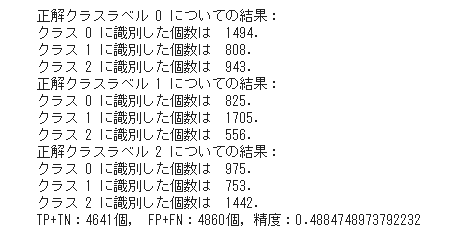
\includegraphics[scale = 1]{1.1.1.png}
  \end{figure}
  \item 混合行列は表\ref{table:19}のようになった。
  \begin{table}[hbtp]
    \centering
    \caption{1.1.1の混合行列}
    \label{table:19}
      \begin{tabular}{|l|c|c|c|}
        \hline
                  & クラス0と推定 & クラス1と推定 & クラス2と推定 \\
        \hline 
        クラス0(P)&     1494 (TP) &       808 (FN) &      943 (FN) \\
        クラス1(N)&      825 (FP) &      1705 (TN) &      556 (FN) \\
        クラス2(N)&      975 (FP) &       753 (FN) &     1442 (TN) \\
        \hline
      \end{tabular}
  \end{table}
\end{itemize}
\clearpage

\hyperlink{holda}{\hypertarget{holda2}{\subsubsection{ホールドアウト法(最初の80\%を学習・残りの20\%をテスト)}}}
\begin{itemize}
  \item スクリプトの出力、精度は図\ref{graph:2}のようになった。
\end{itemize}

\begin{figure}[hbtp]
  \centering
  \caption{1.1.2の出力結果}
  \label{graph:2}
  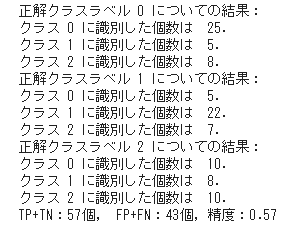
\includegraphics[scale = 1]{1.1.2.png}
\end{figure}

\hyperlink{holdb}{\hypertarget{holdb2}{\subsubsection{ホールドアウト法(最初の20\%をテスト・残りの80\%を学習)}}}
\begin{itemize}
  \item スクリプトの出力、精度は図\ref{graph:3}のようになった。
\end{itemize}

\begin{figure}[hbtp]
  \centering
  \caption{1.1.3の出力結果}
  \label{graph:3}
  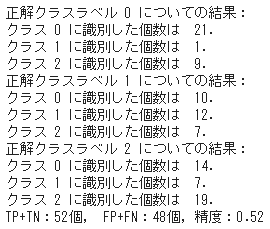
\includegraphics[scale = 1]{1.1.3.png}
\end{figure}
\clearpage

\hyperlink{gobun}{\hypertarget{gobun2}{\subsubsection{5分割の交差確認法}}}
\begin{itemize}
  \item スクリプトの出力、精度はそれぞれ図\ref{graph:4}~\ref{graph:8}のようになった。
  \begin{figure}[htbp]
    \begin{minipage}[t]{0.33\hsize}
      \centering
      \caption{testdata:1~100}
      \label{graph:4}
      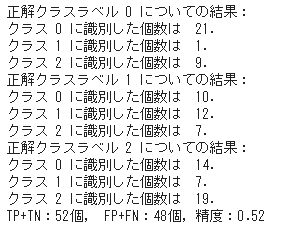
\includegraphics[keepaspectratio, scale=0.7]{test1~100.PNG}
    \end{minipage}
    \begin{minipage}[t]{0.33\hsize}
      \centering
      \caption{testdata:101~200}
      \label{graph:5}
      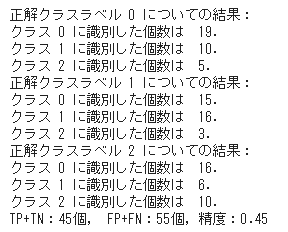
\includegraphics[keepaspectratio, scale=0.7]{test101~200.PNG}
    \end{minipage}
    \begin{minipage}[t]{0.33\hsize}
      \centering
      \caption{testdata:201~300}
      \label{graph:6}
      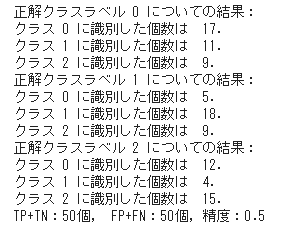
\includegraphics[keepaspectratio, scale=0.7]{test201~300.PNG}
    \end{minipage}
    \begin{minipage}[t]{0.45\hsize}
      \centering
      \caption{testdata:301~400}
      \label{graph:7}
      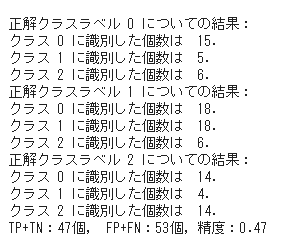
\includegraphics[keepaspectratio, scale=0.7]{test301~400.PNG}
    \end{minipage}
    \begin{minipage}[t]{0.45\hsize}
      \centering
      \caption{testdata:401~500}
      \label{graph:8}
      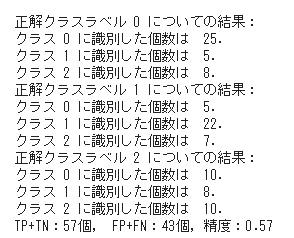
\includegraphics[keepaspectratio, scale=0.7]{test401~500.PNG}
    \end{minipage}
  \end{figure}
  \item 精度を表にまとめると、表\ref{table:20}のようになった。
                            \begin{table}[hbtp]
                              \centering
                              \caption{5分割の交差確認法の精度}
                              \label{table:20}
                                \begin{tabular}{|l|c|}
                                  \hline
                                  testdata  & 精度  \\
                                  \hline
                                  1~100    & 0.52\\
                                  101~100  & 0.45\\
                                  201~100  & 0.50\\
                                  301~100  & 0.47\\
                                  401~100  & 0.57\\
                                  \hline
                                \end{tabular}
                            \end{table}
\LARGE{\item 各試行の結果を平均した精度は、「0.502」となった。}
\end{itemize}
\clearpage

\subsection{課題2}
\hyperlink{hyperpara}{\hypertarget{hyperpara2}{\subsubsection{最近傍法のハイパーパラメータの最適化}}}
\begin{itemize}
  \item 検証データを使った最近傍法のスクリプトの出力、精度はそれぞれ図\ref{graph:9}~\ref{graph:17}のようになった。
  \begin{figure}[htbp]
    \begin{minipage}[t]{0.22\hsize}
      \centering
      \caption{k=1}
      \label{graph:9}
      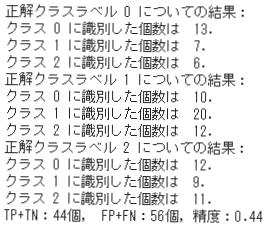
\includegraphics[keepaspectratio, scale=0.6]{k=1.PNG}
    \end{minipage}
    \begin{minipage}[t]{0.22\hsize}
      \centering
      \caption{k=6}
      \label{graph:10}
      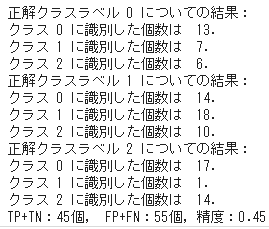
\includegraphics[keepaspectratio, scale=0.6]{k=6.PNG}
    \end{minipage}
    \begin{minipage}[t]{0.22\hsize}
      \centering
      \caption{k=10}
      \label{graph:11}
      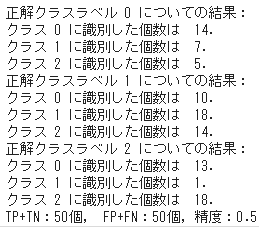
\includegraphics[keepaspectratio, scale=0.6]{k=10.PNG}
    \end{minipage}
    \begin{minipage}[t]{0.22\hsize}
      \centering
      \caption{k=17}
      \label{graph:12}
      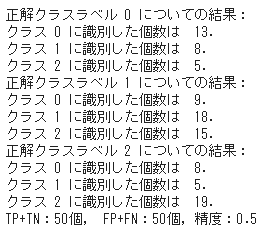
\includegraphics[keepaspectratio, scale=0.6]{k=17.PNG}
    \end{minipage}
    \begin{minipage}[t]{0.22\hsize}
      \centering
      \caption{k=24}
      \label{graph:13}
      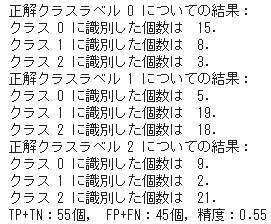
\includegraphics[keepaspectratio, scale=0.6]{k=24.PNG}
    \end{minipage}
    \begin{minipage}[t]{0.22\hsize}
      \centering
      \caption{k=30}
      \label{graph:14}
      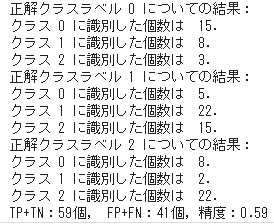
\includegraphics[keepaspectratio, scale=0.6]{k=30.PNG}
    \end{minipage}
    \begin{minipage}[t]{0.22\hsize}
      \centering
      \caption{k=38}
      \label{graph:15}
      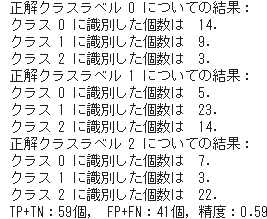
\includegraphics[keepaspectratio, scale=0.6]{k=38.PNG}
    \end{minipage}
    \begin{minipage}[t]{0.22\hsize}
      \centering
      \caption{k=45}
      \label{graph:16}
      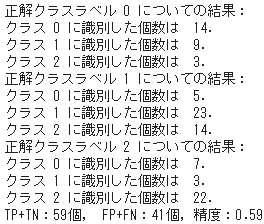
\includegraphics[keepaspectratio, scale=0.6]{k=45.PNG}
    \end{minipage}
    \begin{minipage}[t]{0.22\hsize}
      \centering
      \caption{k=52}
      \label{graph:17}
      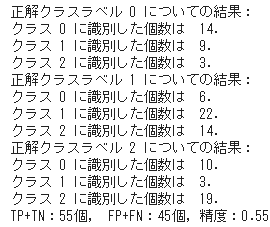
\includegraphics[keepaspectratio, scale=0.6]{k=52.PNG}
    \end{minipage}
    \begin{minipage}[t]{0.78\hsize}
      \centering
      \caption{k=38 テスト結果}
      \label{graph:18}
      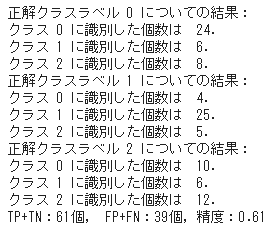
\includegraphics[keepaspectratio, scale=1]{k=38test.PNG}
    \end{minipage}
  \end{figure}
  \LARGE{\item k=30,k=38,k=45の時の精度「0.59」が最も高くなった。
  \item 精度が最も高くなったk=38で、テストデータを使った結果、図\ref{graph:18}のように、精度は「0.61」となった。}
\end{itemize}